\begin{exercise}
      {ID-e5e411dbaf3829361a0b15534a2609be822da2a8}
      {Raumdiagonale}
  \ifproblem\problem
    Berechne die Längen der Diagonalen $d_{ab}$, $d_{ac}$, $d_{bc}$ und $d$.
    \begin{center}
      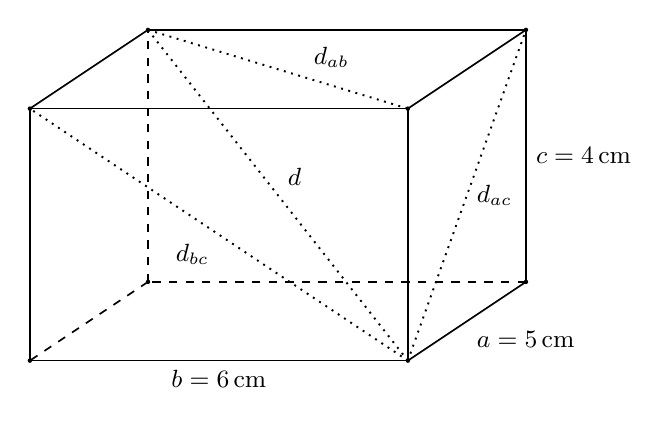
\begin{tikzpicture}[scale=0.8, line width=0.6pt]
        % Punktkoordinaten
        \coordinate (PA) at ( -0.3750,  -0.2500);
        \coordinate (PB) at ( -2.2500,  -1.5000);
        \coordinate (PC) at (  3.7500,  -1.5000);
        \coordinate (PD) at (  5.6250,  -0.2500);
        \coordinate (PE) at ( -0.3750,   3.7500);
        \coordinate (PF) at ( -2.2500,   2.5000);
        \coordinate (PG) at (  3.7500,   2.5000);
        \coordinate (PH) at (  5.6250,   3.7500);
        % Ecken
        \fill (PA) circle (1pt);
        \fill (PB) circle (1pt);
        \fill (PC) circle (1pt);
        \fill (PD) circle (1pt);
        \fill (PE) circle (1pt);
        \fill (PF) circle (1pt);
        \fill (PG) circle (1pt);
        \fill (PH) circle (1pt);
        % Kanten unten
        \draw[dashed] (PA) -- (PB);
        \draw         (PB) -- (PC);
        \draw         (PC) -- (PD);
        \draw[dashed] (PD) -- (PA);
        % Kanten oben
        \draw (PE) -- (PF);
        \draw (PF) -- (PG);
        \draw (PG) -- (PH);
        \draw (PH) -- (PE);
        % Kanten senkrecht
        \draw[dashed] (PA) -- (PE);
        \draw         (PB) -- (PF);
        \draw         (PC) -- (PG);
        \draw         (PD) -- (PH);
        % Diagonalen
        \draw[line width=0.7pt, dotted] (PC) -- (PF);
        \draw[line width=0.7pt, dotted] (PC) -- (PH);
        \draw[line width=0.7pt, dotted] (PE) -- (PG);
        \draw[line width=0.7pt, dotted] (PE) -- (PC);
        % Beschriftung
        \path (PB) -- node[below]       {{\small$b=6\mathrm{\,cm}$}} (PC);
        \path (PC) -- node[below right] {{\small$a=5\mathrm{\,cm}$}} (PD);
        \path (PD) -- node[right]       {{\small$c=4\mathrm{\,cm}$}} (PH);
        \path (PE) -- node[pos=0.6, above right] {{\small$d_{ab}$}}           (PG);
        \path (PC) -- node[below left]  {{\small$d_{bc}$}}           (PF);
        \path (PC) -- node[right]       {{\small$d_{ac}$}}           (PH);
        \path (PC) -- node[above right] {{\small$d$}}                (PE);
      \end{tikzpicture}
    \end{center}
  \fi
  %\ifoutline\outline
  %\fi
  %\ifoutcome\outcome
  %\fi
\end{exercise}
